Tous les codes de cette leçon sont dans le projet \texttt{raytracing-extended} qui est basé sur le projet \texttt{raytracing} implémenté dans la leçon précédente.

\subsection{Question 1}

On va ici pour chaque étape décrire les modifications apportées au code, sans mettre les codes complets, pour les codes complets il suffira de se réferrer aux codes sources.

Dans les modifictions que nous allons apporter au code, nous allons devoir étendre la méthode \texttt{traceRay} de la classe \texttt{RayTracing}. Pour cela nous allons juste après le code qui permets de tester les collisions créer quatre variables qui nous servirons tout au long de ces modifications ;

\begin{lstlisting}
Vector3 ip = Vector3.add(rayPosition, Vector3.multiply(rayDirection, tret));
Vector3 normal = Vector3.normalize(hittedObject.getNormal(ip));
        
ColorRGB finalColor = new ColorRGB(0, 0, 0);
ColorRGB objectColor = hittedObject.getColor(ip);
\end{lstlisting}

\subsubsection{Diffuse reflection and ambient light}

On commence par créer une classe qui représente une lampe.

\code{raytracing-extended}{Lamp.java}

Une \texttt{LinkedList} de lampes est créée au début de \texttt{RayTracing}, ainsi qu'une couleur pour la lumière ambiante.

\begin{lstlisting}
LinkedList<Lamp> lamps=new LinkedList<>();
private ColorRGB ambientLight;
\end{lstlisting}

Dans le constructeur de RayTracing on peut alors ajouter des lampes et définir la couleur de la lumière ambiante.

\begin{lstlisting}
lamps.add(new Lamp(new Vector3(-10, 10, 10), new ColorRGB(0.9, 0.9, 0.9)));
lamps.add(new Lamp(new Vector3(5, 10, 10), new ColorRGB(0.5, 0.5, 0.5)));
ambientLight = new ColorRGB(0.3, 0.3, 0.3);
\end{lstlisting}

Les méthodes \texttt{getNormal} dans les classes représentant les objets avaient déjà été implémentées lors de la leçon précédente. Par exemple, voici la méthode pour la classe \texttt{SphereObject} :

\begin{lstlisting}
public Vector3 getNormal(Vector3 pointOnSurface) {
    Vector3 min = Vector3.subst(pointOnSurface, c);
    return new Vector3(min.x/radius, min.y/radius, min.z/radius);
}
\end{lstlisting}

On peut alors parcourir la liste des lampes pour calculer la couleur. Pour le fonctionnement du code, se réferrer à l'algorithme dans les slides. Pour finir, on ajoute également la lumière ambiante.

\begin{lstlisting}
// ***** Diffuse reflection and ambient light *****
for (int i = 0; i < lamps.size(); i++) {
    Lamp light = lamps.get(i);
    Vector3 dl = Vector3.normalize(Vector3.subst(light.pos, ip));
    double cosa = Vector3.dotProduct(normal, dl)/(Vector3.getLength(normal) * Vector3.getLength(dl));
    if (cosa>0) {
        finalColor.add(ColorRGB.multiply(light.color, objectColor, cosa));
    }
}
finalColor.add(ColorRGB.multiply(ambientLight, objectColor));
\end{lstlisting}

\begin{figure}[H]
	\caption{\label{10_1} Réflexion diffuse et lumière ambiante}
	\centering
	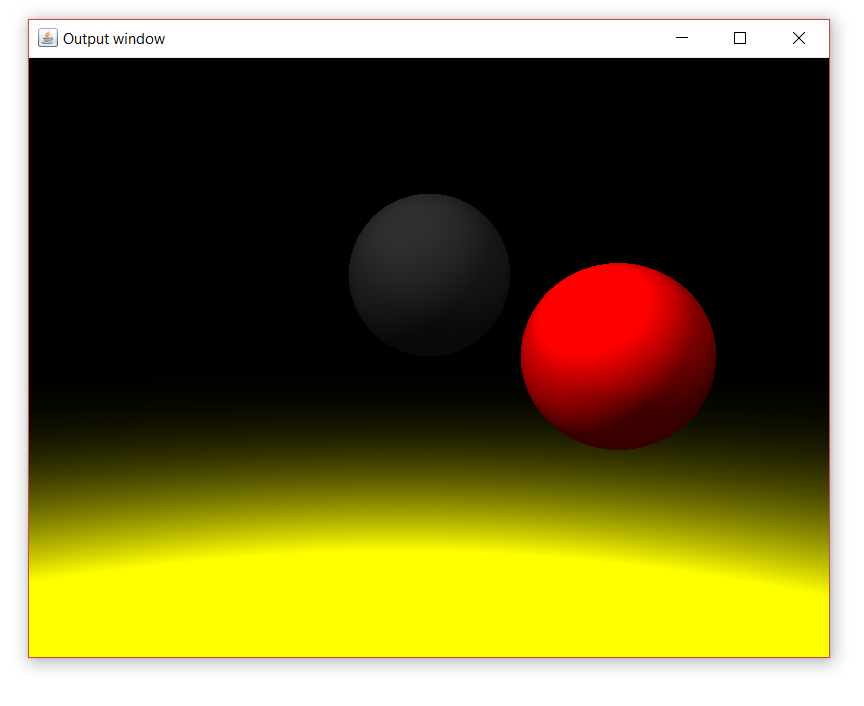
\includegraphics[scale = 0.4]{10_1.png}
\end{figure}

\subsubsection{Shadows}

Pour créer des ombres, il faut que dans le code qu'on vient d'ajouter, la couleur ne soit modifié pour une lampe que si il n'y a aucun objet entre la lampe et l'endroit ou l'on se trouve.

On modifie alors la condition qui devient 

\begin{lstlisting}
if (cosa>0 && !testShadow(ip, dl)) {
\end{lstlisting}

Et dans la classe \texttt{RayTracing} on implémente la méthode \texttt{testShadow}. A nouveau, le fonctionnement de cette méthode est décrit dans les slides.

\begin{lstlisting}
private boolean testShadow(Vector3 pos, Vector3 dl) {
    for (int i = 0; i < objects.size(); i++) {
        RealObject here = objects.get(i);
        double thit = here.testCollision(pos, dl);
        
        if (thit>0) {
            return true;
        }
    }
    return false;
}
\end{lstlisting}

\begin{figure}[H]
	\caption{\label{10_2} Ombres}
	\centering
	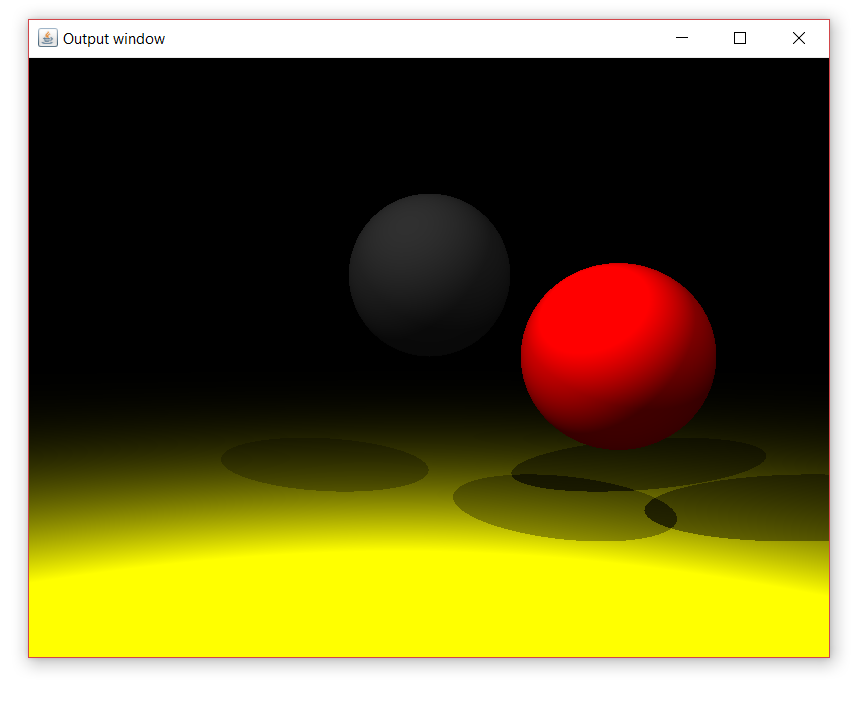
\includegraphics[scale = 0.4]{10_2.png}
\end{figure}

\subsubsection{Perfect reflection}

Pour implémenter la réflexion, on va devoir modifier les classes représentant les objets pour que leurs constructeurs prennent un paramètre qui sera le coefficient de réflection \texttt{kr}. Voici le code ajouté dans la classe \texttt{PlaneObject} (tout le code n'y est pas, ici se trouve uniquement ce qu'on ajoute pour ajouter le coefficient de réflexion)

\begin{lstlisting}
public class PlaneObject extends RealObject {
    public double kr;
    
    public PlaneObject(Vector3 c, Vector3 n, ColorRGB color, double kr) {
        super(color, kr);
        this.c  = c;
        this.n  = n;
        this.kr = kr;
    }
    
    public PlaneObject(Vector3 c, Vector3 n, ColorRGB color) {
        this(c, n, color, 0.);
    }
}
\end{lstlisting}

On modifie également \texttt{RealObject} pour y ajouter ce coefficient :

\begin{lstlisting}
public final ColorRGB color;
public double kr;

public RealObject(ColorRGB color, double kr) {
    this.color=color;
    this.kr = kr;
}
\end{lstlisting}

On peut alors continuer d'étendre la méthode \texttt{traceRay} pour y ajouter une condition qui, si il y a un coefficient de réflexion, va modifier la couleur en conséquence.

\begin{lstlisting}
// ***** Perfect reflexion *****
if (hittedObject.kr>0) { 
    double dn =2*Vector3.dotProduct(rayDirection, normal);
    Vector3 reflectionDirection = Vector3.subst(rayDirection, Vector3.multiply(normal, dn));
    ColorRGB reflection = traceRay(ip, reflectionDirection);
    
    finalColor.add(ColorRGB.multiply(reflection, hittedObject.kr));
}
\end{lstlisting}

\begin{figure}[H]
	\caption{\label{10_3} Réflexion parfaite}
	\centering
	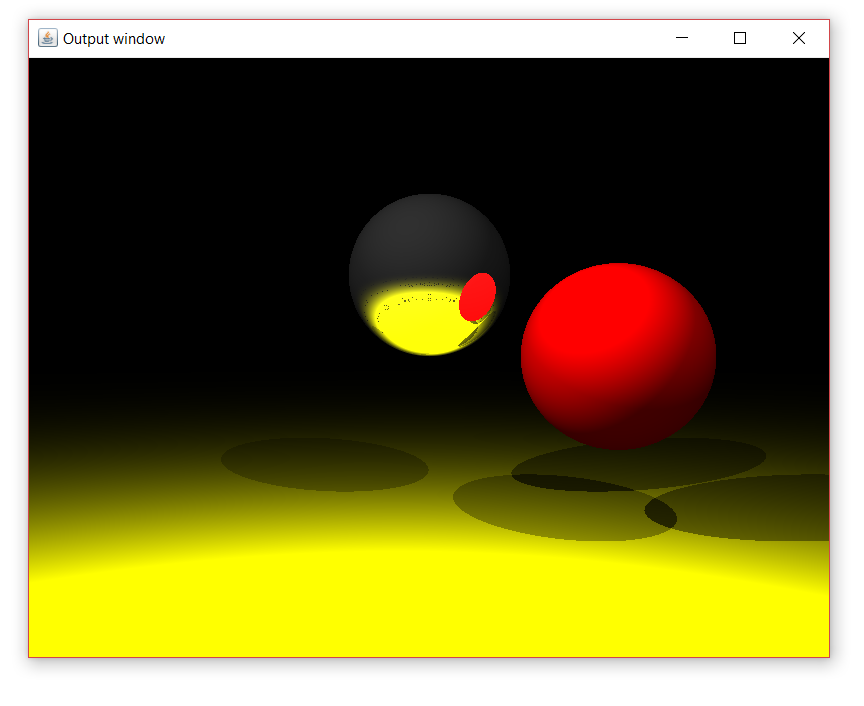
\includegraphics[scale = 0.4]{10_3.png}
\end{figure}

\subsubsection{Texturing}

Pour créer des surfaces avec des textures, on crée une classe \texttt{TexturizedPlaneObject} qui étends \texttt{PlaneObject}.

\code{raytracing-extended}{TexturizedPlaneObject.java}

On peut alors modifier notre scène dans le constructeur

\begin{lstlisting}
objects.add(new PlaneObject(new Vector3(0, -4, 0), new Vector3(0, 1, 0), yellow));
// devient
objects.add(new TexturizedPlaneObject(new Vector3(0, -4, 0), new Vector3(1, 0, 0), new Vector3(0, 0, 1), green));
\end{lstlisting}

\begin{figure}[H]
	\caption{\label{10_4} Textures}
	\centering
	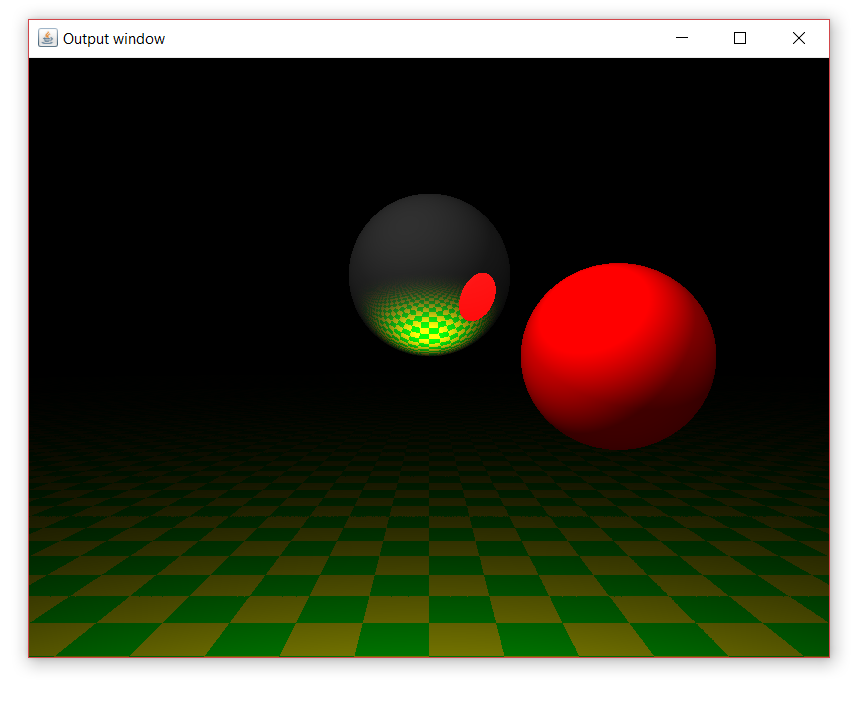
\includegraphics[scale = 0.4]{10_4.png}
\end{figure}

\subsubsection{Parallelograms}

Pour créer des parallèlogrames, on créer une classe \texttt{ParallelogramObject}. Son fonctionnement est semblable au fonctionnement des plans infinis. La principale différence est la méthode \texttt{testCollision} dont le fonctionnement est développé dans les slides.

\code{raytracing-extended}{ParallelogramObject.java}

On peut alors ajouter un parallèlogramme dans notre scène :

\begin{lstlisting}
objects.add(new ParallelogramObject(new Vector3(-5, -1, 0), new Vector3(0, 0, 5), new Vector3(0, 5, 0), green));
\end{lstlisting}

\begin{figure}[H]
	\caption{\label{10_5} Parallèlogrames}
	\centering
	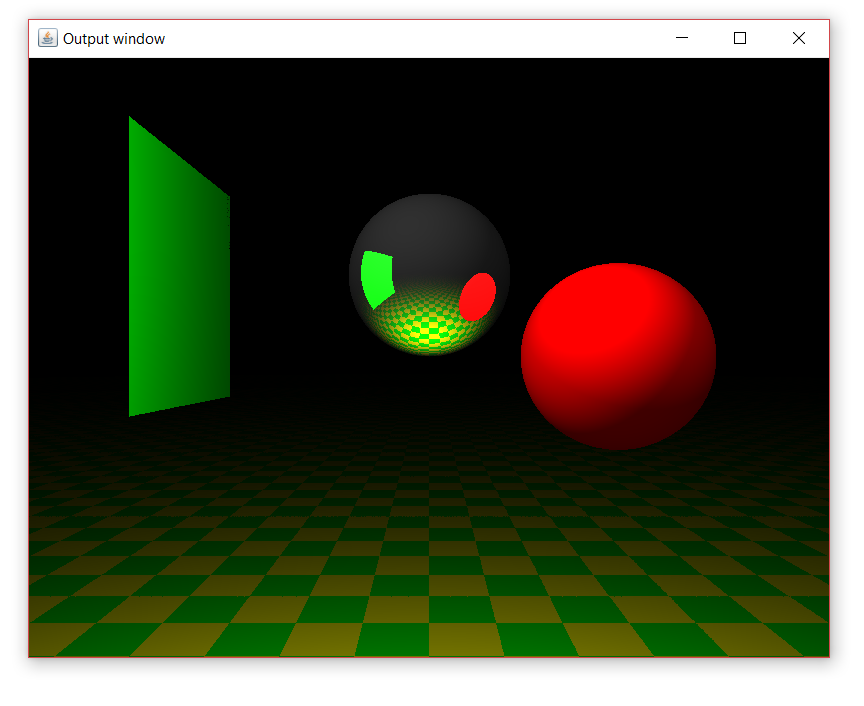
\includegraphics[scale = 0.4]{10_5.png}
\end{figure}

\begin{figure}[H]
	\caption{\label{10_structure} Diagramme de la structure de raytracing-extended}
	\centering
	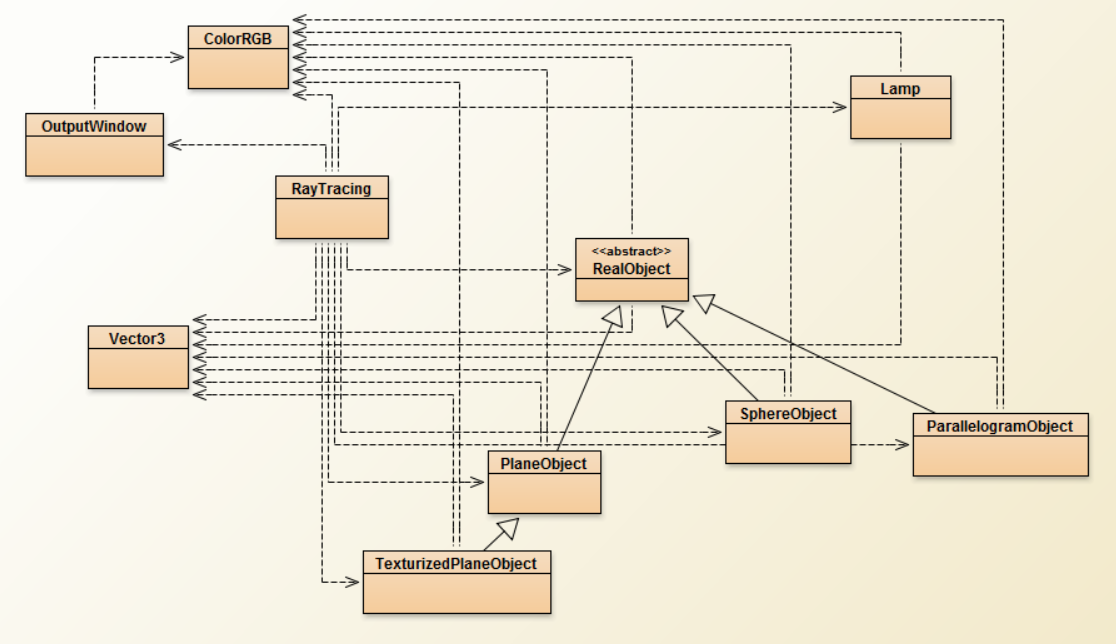
\includegraphics[scale = 0.4]{10_structure.png}
\end{figure}

\subsection{Question 2}

\subsubsection{Point 1}

Parce que si $cos(\alpha)$ est plus petit que $0$, on est déjà sur que la lampe n'a pas d'influence sur l'objet. Il est donc inutile d'appeler la méthode \texttt{testShadow} qui ferais des calculs inutiles.

\subsubsection{Point 2}

Si l'on place plusieurs objetx avec une réflexion parfaite, on peut avoir des réflexions infinies et donc ne jamais s'arrêter. On peut d'une part arrêter de modifier la couleur si elle est déjà totalement blanche, et d'autre part on peut implémenter un compteur qui limite le nombre de réflexions en chaine à calculer.